\chapter[T.d.P. dipendenti dal tempo]{Teoria delle perturbazioni dipendenti dal tempo\footnote{ S5.5,S5.6; LL40,42-44; G21}}
Consideriamo qui le \textbf{perturbazioni dipendenti esplicitamente dal tempo}, in presenza delle quali, cioè, l'hamiltoniano completo ha la forma
\begin{equation}
H=H_0+V(t),
\end{equation}
dove $H_0$ non contiene il tempo esplicitamente. Si assume inoltre risolta l'equazione di Schr\"{o}dinger per $V(t)=0$, nel senso che gli autostati dell'hamiltoniano $H_0$ ed i suoi autovalori, definiti dall'equazione
\begin{equation}
H_0 \vert n ^{(0)} \rangle = E_n ^{(0)} \vert n ^{(0)} \rangle 
\end{equation}
sono noti completamente.\\
Notiamo che, essendo l'hamiltoniano $H$ dipendente dal tempo, non si può più parlare di correzioni agli autovalori dell'energia. \textbf{L'energia non si conserva}, e gli stati stazionari non esistono. Il problema consiste qui nel calcolo approssimato degli stati del sistema nella base degli stati stazionari del sistema imperturbato.\\
Scriviamo lo stato del sistema fisico al tempo $t=0$ come combinaizone lineare di autostati di $H_0$:
\begin{equation}
\vert \alpha ,t=0  \rangle = \sum _k c_k (0) \vert k ^{(0)} \rangle .
\label{eq:cap15_1}
\end{equation}
Lo \textbf{stato del sistema al tempo} $t>0$ potrà allora essere espresso come
\begin{equation}
\vert \alpha ,t  \rangle = \sum _k c_k (t)\ e^{-\frac{i}{\hbar}E_k ^{(0)} t } \vert k ^{(0)} \rangle ,
\label{eq:cap15_2}
\end{equation}
dove la disposizione temporale degli stati stazionari $\vert k ^{(0)} \rangle$, dovuta all'hamiltoniano imperturbato $H_0$, è stata esplicitamente separata dai coefficienti $c_k {(t)}$. In questo modo, l'evoluzione temporale dei coefficienti è dovuta esplicitamente alla presenza della perturbazione $V(t)$. (Si dice che i coefficienti $c_k (t)$ definiscono lo sviluppo del vettore di stato $\vert \alpha , t \rangle $ nella ``rappresentazione di interazione'').\\
I coefficienti $c_k (t)$ soddisfano un insieme di equazioni che può essere ottenuto applicando al vettore di stato $\vert \alpha , t \rangle $ l'equazione di Schr\"{o}dinger dipendente dal tempo:
\begin{eqnarray}
i\hbar \frac{\partial}{\partial t} \vert \alpha , t \rangle &=& \sum _ k \left( i\hbar \frac{dc_k}{dt}+ E_k ^{(0)} c_k\right)e^{-\frac{i}{\hbar}E_k ^{(0)} t } \vert k ^{(0)} \rangle = \nonumber \\
& = & H\vert \alpha , t \rangle  = \left( H_0 + V\right)e^{-\frac{i}{\hbar}E_k ^{(0)} t } \vert k ^{(0)} \rangle  =  \nonumber\\
& = &\sum _k \left( E_k ^{(0)}+ V\right)c_k\ e^{-\frac{i}{\hbar}E_k ^{(0)} t } \vert k ^{(0)} \rangle 
\end{eqnarray}
da cui si ottiene
\begin{equation}
\sum _ k i\hbar \frac{dc_k}{dt} \ e^{-\frac{i}{\hbar}E_k ^{(0)} t } \vert k ^{(0)} \rangle = \sum _ k V c_k\ e^{-\frac{i}{\hbar}E_k ^{(0)} t } \vert k ^{(0)} \rangle .
\end{equation}
Moltiplicando entrambi i membri di questa equazione per il bra $\langle n^{(0)} \vert$ otteniamo infine il \textbf{sistema di equazioni esatte}
\begin{equation}
i\hbar \frac{dc_n (t)}{dt} = \sum _ k V_{nk} (t) c_k\ e^{i\omega _{nk}t } ,
\label{eq:cap15_3}
\end{equation}
dove si è posto
\begin{equation}
\omega _{nk} = \frac{E_n ^{(0})-E_k ^{(0})}{\hbar}
\end{equation}
e $V_{kn} (t)$ sono gli elementi di matrice, dipendenti esplicitamente dal tempo,
\begin{equation}
V_{kn} (t) = \langle n ^{(0)} \vert V(y) \vert k ^{(0)} \rangle .
\end{equation}
Ci proponiamo ora di risolvere le eq. (\ref{eq:cap15_3}) utilizzando la \textbf{teoria delle perturbazioni}. A tale scopo sviluppiamo i coefficienti $c_n (t)$ nella serie
\begin{equation}
c_n (t) = c_n ^{(0)}(t)+c_n ^{(1)}(t)+c_n ^{(2)}(t)+\dots
\end{equation}
dove il generico $c_n ^{(k)}(t)$ è di ordine $k$ nella perturbazione.\\
Sostituendo il precedente sviluppo nell'eq. (\ref{eq:cap15_3}) e considerando i termini di \textbf{ordine zero} si ottiene
\begin{equation}
i\hbar \frac{d c_n ^{(0)}(t)}{dt}=0 ,
\end{equation}
da cui
\begin{equation}
c_n ^{(0)}(t) = \textrm{costante}= c_n ^{(0)} .
\label{eq:cap15_4}
\end{equation}
Questo risultato è consistente con l'aver definito i coefficienti $c_n (t)$ in modo tale che la loro dipendenza esplicita dal tempo sia determinata esplicitamente dalla presenza della perturbazione $V(t)$.\\
Considerando nell'eq. (\ref{eq:cap15_3}) i termini del \textbf{primo ordine} in $V$ si ottiene poi:
\begin{equation}
i\hbar \frac{d c_n ^{(1)}(t)}{dt}=\sum _k V_{nk} (t) c_k (0)\ e^{i\omega _{nk} t}  ,
\end{equation}
avendo sostituito $c_k ^{(0)} (t)$ con $c_k (0)$, in accordo con l'eq. (\ref{eq:cap15_4}). Questa espressione può essere esplicitamente integrata con la condizione al contorno $ c_n ^{(1)} (0) =0$, che segue direttamente dalla (\ref{eq:cap15_4}): $c_n (0) = c_n ^{(0)} (0)$. Si ottiene in tal modo:
\begin{equation}
c_n ^{(1)} (t) = -\frac{i}{\hbar} \sum _k c_k (0) \int _0 ^t dt'\ V_{nk} (t') e ^{i \omega _{nk} t'} ,
\label{eq:cap15_5}
\end{equation}
che determina lo stato del sistema al primo ordine dello sviluppo perturbativo. In molti casi pratici questa approssimazione risulta sufficiente e non ci soffermeremo qui a descrivere i termini di ordine più elevato.\\
Nel seguito considereremo sempre il caso in cui all'istante $t=0$ il sistema si trova in un autostato dell'hamiltoniana imperturbata $H_0$, ossia
\begin{equation}
\vert \alpha , t=0\rangle = \vert i ^{(0)} \rangle \textrm{ e dunque } 
 \begin{cases}
   c_i (0)=1\\c_k (0)=0, \textrm{ per }k\neq i.
   \end{cases}
\end{equation}
In questo caso il modulo quadro del coefficiente $c_n (t)$ fornisce la probabilità che il sistema abbia effettuato, dopo un tempo $t$, una transizione nell'autostato $\vert n^{(0)} \rangle $ di $H_0$:
\begin{equation}
P_{i\rightarrow n} (t) = \vert c_n (t) \vert ^2 = \vert c_n ^{(1)}(t)+c_n ^{(2)}(t)+\dots \vert ^2 ,
\end{equation}
per $n \neq i$. Al primo ordine $P_{i\rightarrow n} (t) \simeq \vert c_n  ^{(1)}(t) \vert ^2$ e l'eq. (\ref{eq:cap15_5}) fornisce semplicemente
\begin{equation}
\vert c_n  ^{(1)}(t) \vert ^2 = \frac{1}{\hbar ^2}\left\vert \int _0 ^t dt'\ V_{ni} (t') e ^{i \omega _{ni} t'} \right\vert ^2
\end{equation}
\section{Transizione per effetto di una perturbazione costante e relazione di indeterminazione tempo-energia}
Il metodo sviluppato è ancora valido quando l'energia di perturbazione $V$ non dipende esplicitamente dal tempo $t$. In questo caso potremmo, se lo volessimo, trattare il sistema  mediante la teoria delle perturbazioni indipendenti dal tempo e trovare i suoi stati stazionari. Tuttavia se ciò che vogliamo calcolare si riferisce esplicitamente al tempo, ad esempio dobbiamo calcolare le probabilità che il sistema si trovi in un certo stato ad un istante determinato, quando sia noto che esso si trovava in un certo stato ad un altro istante, allora il metodo della teoria delle perturbazioni dipendente dal tempo qui considerato risulta più conveniente.\\
Assumiamo dunque
\begin{equation}
V(t) = V \quad \textrm{(indipendente da }t\textrm{),}
\end{equation}
dove l'operatore $V$ è in generale funzione degli operatori impulso, posizione e spin.\\
Assumendo anche, come discusso in precedenza, che al tempo $t=0$ il sistema si trovi nello stato stazionario $\vert i^{(0)}\rangle $ dell'hamiltoniano imperturbato $H_0$, troviamo dall'eq. (\ref{eq:cap15_5}) l'espressione al primo ordine per il coefficiente $c_n (t)$:
\begin{eqnarray}
c_n ^{(1)} (t) & = & -\frac{i}{\hbar} \int _0 ^t dt'\ V_{ni} e^{i \omega _{ni} t'} = \nonumber \\
&=& -\frac{i}{\hbar} V_{ni} \frac{e^{i \omega _{ni} t}-1}{i \omega _{ni}}= -\frac{2i}{\hbar} V_{ni}\ e^{i \omega _{ni} \frac{t}{2}}\ \frac{\sin{\left(\omega _{ni} \frac{t}{2}\right)}}{\omega _{ni}} .
\end{eqnarray}
La probabilità di transizione $i\rightarrow n $, determinata al primo ordine dal modulo quadro $\vert c_n ^{(1)} (t) \vert ^2$, risulta dunque\footnote{Allo stesso risultato si giunge naturalmente utilizzando la teoria delle perturbazioni indipendente dal tempo evolvendo $ \vert \alpha , t =0 \rangle \rightarrow \vert \alpha , t \rangle$} (ricordando che $\omega _{ni} = ( E_n ^{(0)}- E_i ^{(0)})/ \hbar$)
\begin{equation}
\vert c_n ^{(1)} (t) \vert ^2 = \frac{4\vert V_{ni} \vert ^2}{\left( E_n ^{(0)} - E_i ^{(0)} \right) ^2}\ \sin ^2\frac{\left( E_n ^{(0)} - E_i ^{(0)} \right) t}{2 \hbar}.
\label{eq:cap15_6}
\end{equation}
La probabilità di transizione allo stato $\vert n ^{(0)} \rangle$, dunque, oltre ad essere proporzionale all'elemento di matrice modulo quadro $\vert V_{ni}\vert ^2$, dipende dalla differenza delle energie imperturbate $(E_n ^{(0)} - E_i ^{(0)}) $. Per tempi sufficientemente grandi la funzione ha la forma
\begin{figure}[!htbp]
\begin{center}
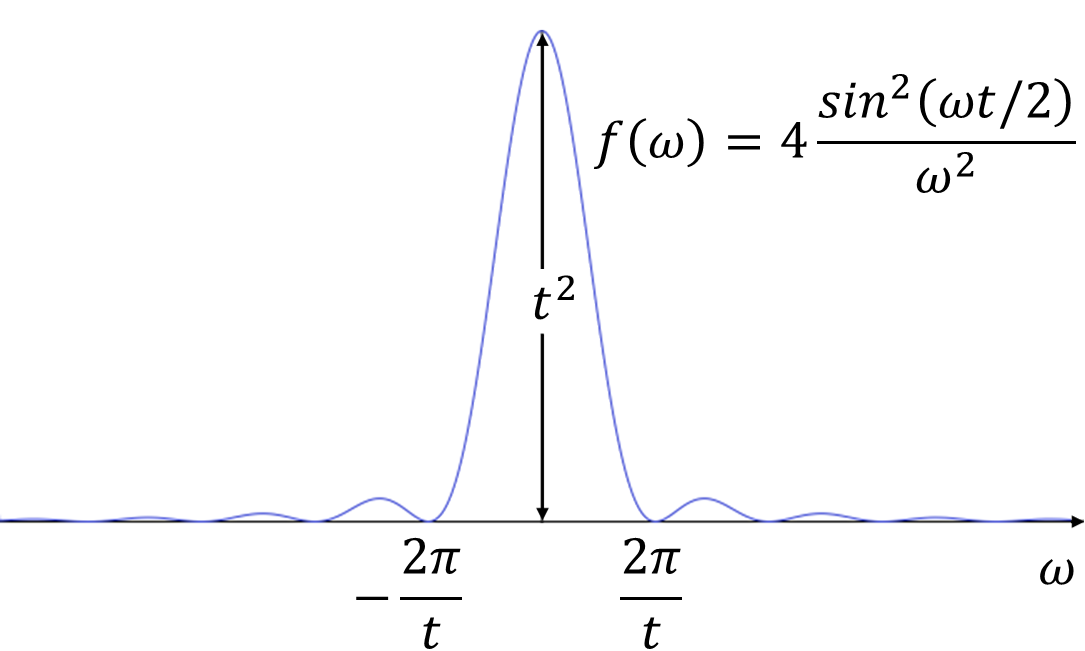
\includegraphics[width=8cm]{immagini/cap_15/fig_15_1.png}
\end{center}
\end{figure}

ossia la probabilità di transizione differisce apprezzabilmente da zero solo per quegli stati finali che soddisfano
\begin{equation}
\vert \omega \vert = \frac{\vert E_n ^{(0)} - E_i ^{(0)}\vert}{\hbar} \leq \frac{2\pi}{t}.
\end{equation}
In altri termini, se indichiamo con $\Delta t$ l'intervallo di tempo durante il quale la perturbazione ha agito sul sistema e con $\Delta E = \vert E_n ^{(0)} - E_i ^{(0)}\vert$ la differenza delle energie imperturbate relativi agli stati finale ed iniziale, si può avere con probabilità apprezzabile una transizione sole se
\begin{equation}
\Delta E \Delta t \sim \hbar .
\label{eq:cap15_7}
\end{equation}
Questa relazione è anche detta \textbf{relazione di indeterminazione tempo-energia}.\\
L'espressione (\ref{eq:cap15_6}) per la probabilità di transizione $i\rightarrow n$ e la condizione (\ref{eq:cap15_7}) che ne segue esprimono il seguente risultato: se $E_n ^{(0)}$ differisce apprezzabilmente da   $E_i ^{(0)}$, la probabilità di transizione $i \rightarrow n$ è piccola e tale rimane per tutti i valori di $t$. Questo risultato è richiesto dalla  \textbf{legge di conservazione dell'energia}. L'energia totale $E$ è costante, perché l'hamiltoniana $H$ non dipende esplicitamente dal tempo, pertanto l'energia propria $E^{(0)}$ (cioè l'energia che si ottiene trascurando la parte $V$ dovuta alla perturbazione), essendo approssimativamente uguale ad $E$, deve essere approssimativamente costante. Ciò significa che se $E^{(0)}$ ha inizialmente il valore $E _i ^{(0)}$, in qualsiasi istante successivo ci deve essere solo una probabilità piccola che esso abbia un valore considerevolmente diverso da $E _i ^{(0)}$.\\
La relazione (\ref{eq:cap15_7}) ci dice anche che un'interazione, sia pure arbitrariamente debole, che agisce per un tempo $\Delta t$, può variare l'energia propria del sistema di una quantità $\Delta E \sim \hbar /\Delta t$.\\
Questo risultato, puramente quantistico, ha un significato fisico profondo. Esso prova che \textbf{nella meccanica quantistica la legge di conservazione dell'energia può essere verificata mediante una misura soltanto a meno di una grandezza dell'ordine di} $\hbar /\Delta t$, \textbf{dove } $\Delta t$ \textbf{è la durata del processo di misura}. Infatti, una sia pur debole interazione tra lo strumento di misura ed il sistema in esame, che agisce per un tempo $\Delta t $, può sempre variare l'energia del sistema di una quantità $\Delta E \sim \hbar /\Delta t$.\\
È utile sottolineare che il \textbf{significato} della relazione (\ref{eq:cap15_7}) è \textbf{essenzialmente diverso da quello della relazione di indeterminazione} $\Delta p \Delta x\sim \hbar$, per la coordinata e la quantità di moto. In quest'ultima $\Delta p$ e $\Delta x$ sono le indeterminazioni nei valori della quantità di moto e della coordinata in uno stesso istante;  essa mostra che queste due grandezze non possono avere contemporaneamente valori esattamente determinati. L'energia $E ^{(0)}$, invece, può essere misurata in ogni istante con la precisione voluta. La grandezza $\Delta E = E_n ^{(0)} - E_i ^{(0)}$ è la differenza di sue valori esattamente misurati dell'energia $E^{(0)}$ in due stati, e non l'indeterminazione nei valori dell'energia in un istante determinato.\\
È utile mostrate che per \textbf{grandi tempi} $t$, \textbf{la probabilità di transizione} $P_{i\rightarrow n} (t) \simeq \vert c_n ^{(1)} (t) \vert ^2$ \textbf{espressa dalla relazione (\ref{eq:cap15_6}), può essere considerata proporzionale a } $t$.\\
A questo scopo osserviamo che vale la formula seguente:
\begin{equation}
\lim _{t \rightarrow \infty} \frac{\sin ^2 (\alpha t)}{\pi t \alpha ^2} = \delta (\alpha),
\label{eq:cap15_8}
\end{equation}
infatti per $\alpha \neq 0$ questo limite è nullo, mentre per  $\alpha = 0$. Si ha $\sin ^2 (\alpha t)/\alpha ^2 t = t$, cosicché il limite è infinito. Integrando poi in $d \alpha$ da $-\infty$ a $+\infty$ si ottiene (sostituendo $\alpha t = \xi$)
\begin{equation}
\frac{1}{\pi t}\int _{-\infty} ^{+\infty} d\alpha \ \frac{\sin ^2 (\alpha t)}{ \alpha ^2} = \frac{1}{\pi}\int _{-\infty} ^{+\infty} d\xi \ \frac{\sin ^2 \xi}{ \xi ^2}=1. 
\end{equation}
In tal modo la funzione a primo membro della (\ref{eq:cap15_8}) soddisfa effettivamente tutte le condizioni che definiscono una funzione $\delta$. Il risultato espresso nell'eq. (\ref{eq:cap15_8}) può essere anche visualizzato dal grafico della funzione $f(\omega)$ presentato in precedenza. Al crescere del tempo $t$ l'altezza del picco centrale della funzione cresce (proporzionalmente a $t^2$) e la sua larghezza decresce (proporzionalmente ad $1/t$). L'integrale della funzione, ossia l'area sottesa dalla curva è proporzionale a $t^2\cdot 1/t =t$, e dunque la funzione $f(\omega)/t$ ha, per grandi $t$, area costante, come richiesto dalla funzione $\delta$.\\
Conformemente a quanto detto, troviamo dall'eq. (\ref{eq:cap15_6}) che \textbf{per grandi tempi}
\begin{equation}
\vert c_n ^{(1)} (t) \vert ^2 \simeq \frac{1}{\hbar ^2} \vert V_{ni} \vert ^2 \pi t\ \delta\left(\frac{E_n ^{(0)}-E_i ^{(0)}}{2\hbar} \right),
\end{equation}
ossia, osservando che $\delta (ax) = \frac{1}{a} \delta (x)$,
\begin{equation}
\vert c_n ^{(1)} (t) \vert ^2 \simeq \frac{2\pi}{\hbar } \vert V_{ni} \vert ^2  t\ \delta (E_n ^{(0)}-E_i ^{(0)} ),
\label{eq:cap15_9}
\end{equation}
che mostra, come anticipato, che la probabilità di transizione cresce linearmente con il tempo $t$.
È consuetudine considerare la \textbf{probabilità di transizione per unità di tempo}, definita come
\begin{equation}
W_{i\rightarrow n} (t) =\frac{d}{dt} P_{i\rightarrow n} (t),
\end{equation}
che è dunque costante per grandi t.\\
Dall'eq. (\ref{eq:cap15_9}) otteniamo allora:
\begin{equation}
W_{i\rightarrow n} (t) = \frac{2\pi}{\hbar } \vert V_{ni} \vert ^2\ \delta (E_n ^{(0)}-E_i ^{(0)} ).
\label{eq:cap15_10}
\end{equation}
Questo risultato,di grande importanza pratica, è chiamato \textbf{regola d'oro di Fermi} (sebbene la teoria perturbativa dipendete dal tempo sia stata di fatto sviluppata da Dirac).		
L'eq. (\ref{eq:cap15_10}) ha particolare rilevanza per le transizioni nello spettro continuo che, praticamente, cono sempre degeneri. In questo caso le probabilità di transizione a tutti i possibili stati finali con energia $E_n ^{(0)}= E_i ^{(0)}$ si ottiene integrando l'eq. (\ref{eq:cap15_10}) con
\begin{equation}
\int dE_n ^{(0)} \ \rho (E_n ^{(0)}),
\end{equation}
dove $\rho (E)$ rappresenta la \textbf{densità degli stati}, ossia il numero di stati nell'intervallo di energia $(E, E+dE)$.
\section{Transizioni per effetto di una perturbazione periodica}
Consideriamo ora le transizioni indotte da una \textbf{perturbazione periodica}, della forma cioè
\begin{equation}
V(t) = Fe^{-i\omega t} + F^+ e ^{i\omega t},
\label{eq:cap15_11}
\end{equation}
dove $F$ è un operatore non dipendente dal tempo (funzione in generale degli operatori impulso, posizione e spin). Osserviamo che $V(t)$ è un operatore hermitiano, come deve essere.		
Assumendo ancora che al tempo $t=0$ il sistema si trovi nell'autostato $\vert i ^{(0)}\rangle$ dell'hamiltoniano imperturbato $H_0$ (per cui $c_k (0) = \delta _{ik}$ e sostituendo il potenziale (\ref{eq:cap15_11}) nella (\ref{eq:cap15_5}), si ricava:
\begin{eqnarray}
c_n ^{(1)}(t) & = & -\frac{i}{\hbar}\int _0 ^t dt'\ V_{ni} (t') \ e^{i\omega _{ni}t'} = \nonumber \\
&=& -\frac{i}{\hbar}\int _0 ^t dt'\left[ F_{ni}\ e^{i(\omega _{ni}-\omega) t'} + F_{ni} ^+\ e ^{i(\omega _{ni} +\omega) t}\right] = \nonumber \\
&=& -\frac{i}{\hbar}\left[ F_{ni}\ \frac{e^{i(\omega _{ni}-\omega) t}-1}{i(\omega _{ni}-\omega)} + F_{ni} ^+\ \frac{e ^{i(\omega _{ni} +\omega) t}-1}{i(\omega _{ni}+\omega)}\right], 
\end{eqnarray}
ossia
\begin{eqnarray}
c_n ^{(1)}(t)&=&-\frac{2i}{\hbar}\left[ F_{ni}\ e^{i\frac{(\omega _{ni}-\omega) t}{2}}\frac{\sin(\frac{(\omega _{ni}-\omega) t}{2})}{(\omega _{ni}-\omega)} +\right. \nonumber \\
& &\left. + F_{ni} ^+\ e^{i\frac{(\omega _{ni}+\omega) t}{2}}\frac{\sin(\frac{(\omega _{ni}+\omega) t}{2})}{(\omega _{ni}+\omega)}\right].
\label{eq:cap15_12}
\end{eqnarray}
Dai risultati del paragrafo precedente è evidente che, nel calcolo delle probabilità di transizione $\vert c_n ^{(1)}(t)\vert ^2$, il primo termine della (\ref{eq:cap15_12}) fornisce, per tempi grandi, un contributo significativo solo alle transizioni verso quegli stati con energia $E_n ^{(0)} \simeq E_i ^{(0)}+ \hbar \omega $, tali cioè che la differenza  $\omega _{ni} - \omega$ sia piccola. Analogamente il secondo termine della (\ref{eq:cap15_12}) fornisce un contributo significativo solo per le transizioni verso quegli stati con energia  $E_n ^{(0)} \simeq E_i ^{(0)}- \hbar \omega $, per i quali cioè la somma $\omega _{ni} + \omega$ è piccola. Infine  il termine di ``doppio prodotto'' nel calcolo di  $\vert c_n ^{(1)}(t)\vert ^2$ fornisce un contributo che è sempre trascurabile nel limite di tempi grandi, giacché le due condizioni $\omega _{ni} - \omega\simeq 0$ e $\omega _{ni} + \omega\simeq 0$ non sono mai simultaneamente verificate.\\
Dai risultati del paragrafo precedente possiamo ottenere direttamente l'espressione delle \textbf{probabilità di transizione per unità di tempo} valida nel limite di grandi $t$:
\begin{eqnarray}
W_{i\rightarrow n} &=& \frac{2\pi}{\hbar}\left[ \vert F_{ni}\vert ^2 \ \delta (E_n^{(0)}-E_i^{(0)}-\hbar \omega) + \right.\nonumber \\
& &\left. +\vert F_{ni} ^+\vert ^2 \ \delta (E_n^{(0)}-E_i^{(0)}+\hbar \omega)\right],
\label{eq:cap15_13}
\end{eqnarray}
in accordo nuovamente con la \textbf{regolo d'oro di Fermi}.\\
Il significato fisico dei due termini nell'eq. (\ref{eq:cap15_13}) è evidente. Il primo termine corrisponde alle transizioni verso quegli stati, tipicamente nello spettro del continuo, la cui energia $E_n ^{(0)}$ è accresciuta rispetto all'energia dello stato iniziale di una quantità $\hbar \omega$. Questo termine descrive dunque \textbf{l'assorbimento da parte del sistema di una quantità di energia $\hbar \omega$ dal potenziale periodico $V$}. Il secondo termine della (\ref{eq:cap15_13}) corrisponde invece alle transizioni verso quegli stati la cui energia $E_n ^{(0)}$ è minore di una quantità $\hbar \omega$ rispetto all'energia dello stato iniziale $E_i ^{(0)}$. Questo termine descrive il cosiddetto processo di \textbf{emissione stimolata, in cui il sistema cede una quantità $\hbar \omega$ della sua energia al campo esterno $V$. Così una perturbazione dipendente dal tempo può essere vista come una inesauribile sorgente o pozzo di energia}.\\
I due processi di assorbimento ed emissione stimolato posso essere schematicamente rappresentati nel modo seguente:
\begin{figure}[!htbp]
\begin{center}
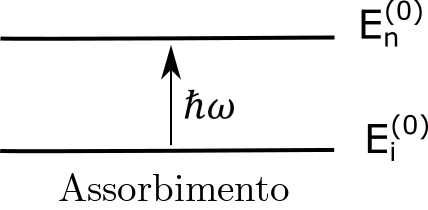
\includegraphics[width=6cm]{immagini/cap_15/fig_15_2.png}\hspace{1cm}
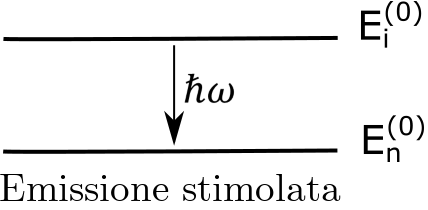
\includegraphics[width=6cm]{immagini/cap_15/fig_15_3.png}
\end{center}
\end{figure}
\newpage
\section*{Appendice al capitolo - I}
Determiniamo l'integrale
\begin{equation}
I= \int _{-\infty} ^{-\infty} dx\ \frac{\sin ^2 x}{x^2}.
\end{equation}
in primo luogo trasformiamo l'integrale con una integrazione per parti:
\begin{eqnarray}
I &=& \int _{-\infty} ^{-\infty} dx\ \frac{d}{dx}\left(\frac{1}{x}\right)\sin ^2 x = \nonumber \\
&=& \left. \frac{1}{x}\sin ^2 x\right\vert _{-\infty} ^{-\infty} +\int _{-\infty} ^{-\infty} dx\ \frac{1}{x} 2 \sin x \cos x =\\
&=& \int _{-\infty} ^{-\infty} dx\ \frac{\sin 2 x}{x}, \nonumber
\end{eqnarray}
ossia
\begin{equation}
I= \int _{-\infty} ^{-\infty} dx\ \frac{\sin  x}{x}. \quad \textrm{[Integrale di Dirichelet]}
\end{equation}
Possiamo poi trasformare l'integrale in un integrale nel piano complesso:
\begin{equation}
I= \int _{-\infty} ^{-\infty} dx\ \frac{\sin  x}{x}= \textrm{Im}\left\{\textrm{PV} \int _{-\infty} ^{-\infty} dz\ \frac{e^{iz}}{z}\right\},
\label{eq:cap15_14}
\end{equation}
dove PV indica il valor principale (la parte reale dell'integrale non è altrimenti definita per il polo in $z=0$). Per calcolare l'integrale scegliamo il seguente contorno:
\begin{figure}[!htbp]
\begin{center}
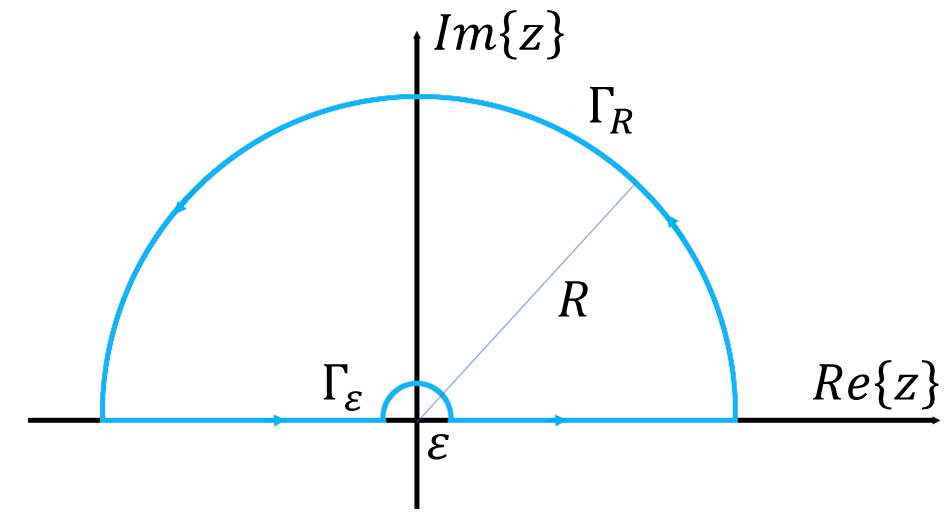
\includegraphics[width=8cm]{immagini/cap_15/fig_15_4.png}
\end{center}
\end{figure}
poiché la funzione integranda non ha poli all'interno del contorno possiamo scrivere:
\begin{eqnarray}
0 & = & \oint  dz\ \frac{e^{iz}}{z} = \nonumber \\
&=& \lim _{R\rightarrow \infty} \lim _{\varepsilon\rightarrow 0} \left[ \int _{-R} ^{-\varepsilon}dz\ \frac{e^{iz}}{z}+\int _{\varepsilon} ^{R}dz\ \frac{e^{iz}}{z}+\int _{\Gamma _{\varepsilon}} dz\ \frac{e^{iz}}{z} +\int _{\Gamma _{R}} dz\ \frac{e^{iz}}{z}\right] = \nonumber\\
&= &\textrm{PV}\int _{-\infty} ^{+\infty}dz\ \frac{e^{iz}}{z}+ \lim _{\varepsilon\rightarrow 0}  \int _{\Gamma _{\varepsilon}} dz\ \frac{e^{iz}}{z}+\lim _{R\rightarrow \infty}\int _{\Gamma _{R}} dz\ \frac{e^{iz}}{z}.
\label{eq:cap15_15}
\end{eqnarray}
L'integrale sul semicerchio esterno tende evidentemente a zero nel limite $R\rightarrow \infty $:
\begin{eqnarray}
\int _{\Gamma _{R}} dz\ \frac{e^{iz}}{z} &\overset{z= Re^{i\varphi}}{=}& \int _0 ^{\pi} d\varphi \ i R e^{i\varphi}\ \frac{e^{iRe^{i\varphi}}}{Re^{i\varphi}} = \nonumber\\
&=&i\int _0 ^{\pi} d\varphi \ e^{iRe^{i\varphi}} \underset{R\rightarrow \infty}{\longrightarrow}0.
\end{eqnarray}
L'integrale su $\Gamma _{\varepsilon}$ dà invece contributo non nullo:
\begin{eqnarray}
\int _{\Gamma _{\varepsilon}} dz\ \frac{e^{iz}}{z} &\overset{z= \varepsilon e^{i\varphi}}{=} &\int _0 ^{\pi} d\varphi \ i \varepsilon e^{i\varphi}\ \frac{e^{i\varepsilon e^{i\varphi}}}{\varepsilon e^{i\varphi}} = \nonumber\\
&=&i\int _0 ^{\pi} d\varphi \ e^{i\varepsilon e^{i\varphi}} \underset{\varepsilon\rightarrow 0}{\longrightarrow}i\int _0 ^{\pi} d\varphi = -i\pi.
\end{eqnarray}
Sostituendo questo risultato nella (\ref{eq:cap15_15}) si ottiene
\begin{equation}
\textrm{PV} \int _{-\infty} ^{-\infty} dz\ \frac{e^{iz}}{z} =-\lim _{\varepsilon \rightarrow 0} \int _{\Gamma _{\varepsilon}} dz\ \frac{e^{iz}}{z}= +i\pi.
\end{equation}
L'eq. (\ref{eq:cap15_14}) implica allora:
\begin{equation}
I= \int _{-\infty} ^{-\infty} dx\ \frac{\sin ^2  x}{x^2}= \int _{-\infty} ^{-\infty} dx\ \frac{\sin  x}{x}= \pi
\end{equation}
\newpage
\section*{Appendice al capitolo - II}
Determiniamo l'espressione per i coefficienti $c_n(t)$ al secondo ordine della teoria delle perturbazioni. L'eq. (\ref{eq:cap15_3}) comporta:
\begin{equation}
i\hbar \frac{dc_n ^{(2)} (t)}{dt} = \sum _k V_{nk} (t)\ c_k ^{(1)}(t) e^{i\omega _{nk}t},
\end{equation}
che può essere direttamente integrata, con la condizione iniziale $c_n ^{(2)} (0)=0 $, per dare:
\begin{equation}
c_n ^{(2)} (t)= -\frac{i}{\hbar}\sum _k \int _0 ^t dt'\ V_{nk} (t')\ c_k ^{(1)} (t') e ^{i\omega _{nk} t'}.
\end{equation}
Sostituendo quindi in questa espressione il risultato (\ref{eq:cap15_5}) per i coefficienti al primo ordine si ottiene dunque
\begin{equation}
c_n ^{(2)} (t)= \left(-\frac{i}{\hbar}\right)^2 \sum _{k,k'} \int _0 ^t dt'\ V_{nk} (t')\ c_k ^{(1)} (t') e ^{i\omega _{nk} t'}\int _0 ^t dt''\ V_{kk'} (t'')\  e ^{i\omega _{kk'} t''}\ c_{k'} ^{(1)} (0).
\end{equation}